\vspace*{1em}

\begin{proposition}[Arguments of Products]\label{prodarg}
Let $z,w$ be non-zero complex numbers, then
\begin{itemize}
\item[(1)] $\arg (zw) = \arg z + \arg w$
\item[(2)] $\arg w^{-1} = -\arg w$
\end{itemize}
\emph{Note that this is \emph{not} saying $\parg(zw) = \parg z + \parg w$, this is actually not true, we're claiming an equality of sets. (1) and (2) together give us $\arg (z/w) = \arg z - \arg w$.}
\end{proposition}
\begin{proof}\hfill
\begin{itemize}
\item[(1)] Consider $\theta \in \arg z$ and $\phi \in \arg w$, so $z = re^{i\theta}$ and $w = se^{i\phi}$. By Proposition \ref{propeuler} (1), we have $zw = rs\ e^{i(\theta + \phi)}$ and therefore $\theta + \phi \in \arg(zw)$. Hence $\arg z + \arg w \subseteq \arg(z + w)$.\\[0.5em]
Consider $\psi \in \arg(z+w)$, and some $\theta \in \arg z$ then we claim that $\psi - \theta \in \arg w$. We have $rs\ e^{i\psi} = zw = re^{i\theta}w$, then by Proposition \ref{propeuler} (5), we get $w = sr^{i(\psi - \theta)}$. Hence $\psi - \theta \in \arg w$, and since $\psi = \theta + (\psi - \theta) \in \arg z + \arg w$, we have $\arg(z+w) \subseteq \arg z + \arg w$.\\[0.5em]
Therefore $\arg (zw) = \arg z + \arg w$.
\item[(2)] Consider $\theta \in \arg z$, so $z = re^{i\theta}$. By Proposition \ref{propeuler} (2), we have $z^{-1} = (1/r)e^{i(-\theta)}$ and therefore $-\theta \in \arg w^{-1}$. Hence $-\arg w \subseteq \arg w^{-1}$.\\[0.5em]
Note that $w = (w^{-1})^{-1}$, applying the above result to $w^{-1}$ gets us $-\arg w^{-1} \subseteq \arg (w^{-1})^{-1} = \arg w$ and so $\arg w^{-1} \subseteq - \arg w$.\\[0.5em]
Therefore $\arg w^{-1} = -\arg w$.
\end{itemize}
\vspace*{-\baselineskip}
\end{proof}

\vspace*{1em}

\begin{remark}
For a complex number, $\arg z$ is a set of all possible $\theta$'s such that we can write $z = \abs{z}e^{i\theta}$, as you know. Therefore, we will abuse notation by sometimes calling any $\theta \in \arg z$ as an argument of $z$, and sometimes also writing $z = \abs{z}e^{i\arg z}$. That is, we are not, or are careless about, distinguishing the set $\arg z$ and its element when we can be agnostic about the choice of $\theta$; for example, the polar form of a complex number. It will be clear when we choose to care about out choice, it will be evident because we'll be then forcing $\theta$ to lie in an interval of length $2\pi$; for example, the principal argument $-\pi < \parg z \leq \pi$.
\end{remark}

\vspace*{1em}

\begin{example}\hfill
\begin{itemize}
\item[(1)] The principal argument of $z = (\sqrt{3} - i)^6$. We first note that $\parg(\sqrt{3} - i) = -\pi/6$. By Proposition \ref{prodarg} (1), applied inductively, we have
\begin{align*}
\arg (\sqrt{3} - i)^6 &= \underbrace{\arg(\sqrt{3} - i) + \cdots + \arg(\sqrt{3} - i)}_{\text{$6$ times}} = \setp{-\pi + 2k\pi}{k \in \zz}
\end{align*}
Then $\parg(\sqrt{3} - i)^6$ is the element in the set above in the interval $(-\pi,\pi]$ which is $\pi$.
\item[(2)] As mentioned previously, we can't just replace $\arg$ with $\parg$ in the statement of Proposition \ref{prodarg} (1). Here's a simple example: let $z = w = -1$, then $\parg z = \parg w = \pi$ and $\parg zw = \parg 1 = 0$ but $0 \neq 2\pi = \parg z + \parg w$.
\item[(3)] Note that $\arg z + \arg z \neq 2\arg z$.
\end{itemize}
\vspace*{-\baselineskip}
\end{example}

%\vspace*{2em}

\begin{mdframed}
\begin{center}
{\Large Roots of Complex Numbers}
\end{center}
\end{mdframed}

\begin{lemma}\label{polareq}
Two non-zero complex numbers $z,w$ are equal if and only if $\abs{z} = \abs{w}$ and $\arg z = \arg w$.
\end{lemma}
\begin{proof}
If $\abs{z} = \abs{w}$ and $\arg z = \arg w$, then clearly $z = w$.\\[0.5em]
Suppose $z = w$, then we immediately get $\abs{z} = \abs{w}$. Consider $\theta \in \arg z$ and $\phi \in \arg w$, then we get $e^{i\theta} = e^{i\phi}$ which is equivalent to saying $\cos(\theta - \phi) + i\sin(\theta - \phi) = e^{i(\theta - \phi)} = 1$. This gives us
\[\sin (\theta - \phi) = 0.\]
The solution to this is $\theta - \phi = 2k\pi$ for some $k\in \zz$. This gives us $\arg z = \arg w$.
\end{proof}

\vspace*{1em}

\begin{definition}[Roots]
Let $\alpha$ be a non-zero complex number. An \emph{$n^{\text{th}}$ root of $\alpha$} is a solution to the polynomial equation $z^n - \alpha = 0$.\\
\\
The set of all $n^{\text{th}}$ roots of $\alpha$ is denoted by $\alpha^{1/n}$, we reserve the symbol $\sqrt[n]{\ \cdot\ }$ for the unique positive $n^{\text{th}}$ root of a positive real number.
\end{definition}

\vspace*{1em}

\begin{proposition}[Distinct Roots]\label{distroot}
There are precisely $n$ distinct $n^{\text{th}}$ roots of $\alpha$, namely
\[\beta_k = \sqrt[n]{\abs{\alpha}}\ e^{i\left(\frac{\parg \alpha}{n} + \frac{2k\pi}{n}\right)},\quad k = 0,\ldots,n-1\]
\end{proposition}
\begin{proof}
Let $z = re^{i\theta}$ and $\alpha = \abs{\alpha}e^{i\parg\alpha}$, we solve
\[r^ne^{in\theta} = z^n = \alpha = \abs{\alpha}e^{i\parg\alpha}.\]
By Lemma \ref{polareq}, this equality is true if and only if $r^n = \abs{\alpha}$ and $n\theta = \parg\alpha + 2k\pi$ for some $k \in \zz$. Therefore
\[z = \sqrt[n]{\abs{\alpha}}\ e^{i\left(\frac{\parg \alpha}{n} + \frac{2k\pi}{n}\right)},\quad k \in \zz\]
We obtain distinct $n$ complex numbers for $k = 0,\ldots,n-1$ since they have distinct arguments, and they necessarily give us the $n$ distinct $n^{\text{th}}$ roots of $\alpha$.
\end{proof}

\vspace*{1em}

\begin{discussion}
With the notation of Proposition \ref{distroot}, the {\color{blue}$n^{\text{th}}$} \cdef{principal\ root\ of} {\color{blue}$\alpha$} is
\[\beta_0 = \sqrt[n]{\abs{\alpha}}\ e^{i\frac{\parg \alpha}{n}}\]
If we introduce the notation $\zeta_n = e^{\frac{2\pi i}{n}}$, then
\[\zeta_n^k = e^{\frac{2k\pi i}{n}}\]
According to the proposition, the complex numbers
\[1,\ \zeta_n,\ \zeta_n^2,\ldots,\zeta_n^{n-1}\]
are the distinct solutions to $z^n - 1 = 0$, the {\color{blue}$n^{\text{th}}$} \cdef{roots\ of\ unity}, making $\zeta_n$ the \emph{principal $n^{\text{th}}$ root of unity}.\\
\\
Then we can write the roots of $\alpha$ in terms of the principal root and the roots of unity
\[\beta_k = \sqrt[n]{\abs{\alpha}}\ e^{i\left(\frac{\parg \alpha}{n} + \frac{2k\pi}{n}\right)} = \sqrt[n]{\abs{\alpha}}\ e^{i\frac{\parg \alpha}{n}}e^{\frac{2k\pi i}{n}}  = \beta_0\zeta_n^k\]
That is, $\beta_k$'s all lie on the circle of radius $\sqrt[n]{\abs{\alpha}}$ centered at the origin, and all of them are obtained by rotating $\beta_0$ by an angle of $2k\pi/n$. That is, they all lie on the vertices of an inscribed regular $n$-gon.
\[\begin{tikzpicture}
    \draw[<->,thick] (-2.5,0)--(2.5,0);
	\draw[<->,thick] (0,-3)--(0,3);
    \draw[thick](0,0) circle (2);
    \draw[->,>=stealth,thick,firebrick](0,0)--(-0.41,1.958);
    \draw[->,>=stealth,thick,firebrick](0,0)--(-1.4,1.428);
    \fill[firebrick] (-0.41,1.958) circle (2pt) node[above]{\color{firebrick}$\beta_{k-1}$};
    \fill[firebrick] (-1.4,1.428) circle (2pt) node[above left]{\color{firebrick}$\beta_{k}$};
    \node (a) at (-1.4,1.428) {};
    \node (b) at (0,0) {};
    \node (c) at (-0.41,1.958) {};
    \draw[->,>=stealth,thick,firebrick](0,0)--(1.73,1.004) node[midway,above,sloped]{\color{firebrick}$\sqrt[n]{\abs{\alpha}}$};
    \fill[firebrick] (1.73,1.004) circle (2pt) node[above right]{\color{firebrick}$\beta_0$};
    \draw pic["{\scriptsize$\color{firebrick}\ \dfrac{2\pi}{n}$}", ->,>=stealth,thick,draw=firebrick, angle eccentricity=1.4, angle radius=1cm] {angle=c--b--a};
  \end{tikzpicture}\]
\end{discussion}

\vspace*{1em}

\begin{example}\hfill
\begin{itemize}
\item[(1)] We compute explicitly the $4^{\text{th}}$ roots of $\alpha = -16$. As a negative real number, $\parg(-16) = \pi$, so
\begin{align*}
\beta_k &= \sqrt[4]{16}e^{i\left(\frac{\pi}{4}+\frac{2k\pi}{4}\right)} = 2\ e^{i\frac{\pi}{4}}e^{\frac{ki\pi}{2}}\\[0.5em]
&= 2\ e^{i\frac{\pi}{4}}\left(e^{\frac{i\pi}{2}}\right)^k\\[0.5em]
&= 2\ \left(\cos\frac{\pi}{4} + i\sin\frac{\pi}{4}\right)\left(\cos\frac{\pi}{2} + i\sin\frac{\pi}{2}\right)^k = 2\ \left(\frac{1}{\sqrt{2}} + i\frac{1}{\sqrt{2}}\right)i^k = \sqrt{2}(1 + i)i^k
\end{align*}
Therefore
\[\begin{tikzpicture}
    \draw[<->,thick] (-2.5,0)--(2.5,0);
	\draw[<->,thick] (0,-2.5)--(0,2.5);
    \draw[thick](0,0) circle (2);
    \draw[->,>=stealth,thick,indigo](0,0)--(1.414,1.414) node[above, midway, sloped]{\color{indigo}$2$};
    \draw[thick,indigo,dashed](1.414,1.414)--(1.414,-1.414);
    \draw[thick,indigo,dashed](1.414,-1.414)--(-1.414,-1.414);
    \draw[thick,indigo,dashed](-1.414,-1.414)--(-1.414,1.414);
    \draw[thick,indigo,dashed](-1.414,1.414)--(1.414,1.414);
    \fill[indigo] (1.414,1.414) circle (2pt) node[above right]{\color{indigo}$\sqrt{2}(1 + i)$};
    \fill[indigo] (1.414,-1.414) circle (2pt) node[below right]{\color{indigo}$\sqrt{2}(1 - i)$};
    \fill[indigo] (-1.414,1.414) circle (2pt) node[above left]{\color{indigo}$\sqrt{2}(-1 + i)$};
    \fill[indigo] (-1.414,-1.414) circle (2pt) node[below left]{\color{indigo}$\sqrt{2}(-1 - i)$};
    \node (a) at (1.414,1.414) {};
    \node (b) at (0,0) {};
    \node (c) at (2,0) {};
    \draw pic["{\scriptsize$\color{indigo}\ \dfrac{\pi}{4}$}", ->,>=stealth,thick,draw=indigo, angle eccentricity=1.25, angle radius=1cm] {angle=c--b--a};
  \end{tikzpicture}\]
\[\beta_0 = \sqrt{2}(1 + i),\quad \beta_1 = \sqrt{2}(-1 + i),\quad \beta_2 = \sqrt{2}(-1-i),\quad \beta_3 = \sqrt{2}(1-i)\]
\item[(2)] In the course of the previous example, we have computed the $4^{\text{th}}$ roots of unity, since they are
\[e^{\frac{2ki\pi}{4}} = e^{\frac{ki\pi}{2}},\quad k = 0,1,2,3\]
as $\parg 1 = 0$. Letting $\zeta_4 = e^{i\pi/2} = i$, the $4^{\text{th}}$ roots of unity are $\zeta_4^0,\zeta_4^1,\zeta_4^2,\zeta_4^3$, which are nothing but $\pm 1,\pm i$.
\end{itemize}
\end{example}

\vspace*{1em}

\begin{example}[in-class]\label{cuberootofunity}
Compute the $3^{\text{rd}}$ roots of unity, also called the cube roots of unity where we denote $\omega = \zeta_3$, explicitly.
\[\begin{tikzpicture}[scale=0.9]
    \draw[<->,thick] (-3,0)--(3,0);
	\draw[<->,thick] (0,-3)--(0,3);
    \draw[thick](0,0) circle (2);
    \draw[->,>=stealth,thick,dirt](0,0)--(-1,1.732);
    \draw[thick,dirt,dashed](2,0)--(-1,1.732);
    \draw[thick,dirt,dashed](-1,1.732)--(-1,-1.732);
    \draw[thick,dirt,dashed](-1,-1.732)--(2,0);
    \fill[dirt] (-1,1.732) circle (2pt) node[above left]{\color{dirt}$\omega$};
    \fill[dirt] (-1,-1.732) circle (2pt) node[below left]{\color{dirt}$\omega^2$};
    \fill[dirt] (2,0) circle (2pt) node[below right]{\color{dirt}$1$};
    \node (a) at (-1,1.732) {};
    \node (b) at (0,0) {};
    \node (c) at (2,0) {};
    \draw pic["{\ \ \tiny$\color{dirt}\ \dfrac{2\pi}{3}$}", ->,>=stealth,thick,draw=dirt, angle eccentricity=1.6, angle radius=0.3cm] {angle=c--b--a};
  \end{tikzpicture}\]
\end{example}
\begin{proof}[Answer]
Let the principal root be $\omega = \zeta_3$, then the cube roots of unity are
\[1,\ \omega,\ \omega^2\]
where we have
\begin{align*}
\omega = e^{\frac{2\pi i}{3}} &= \left(\cos\frac{2\pi}{3} + i\sin\frac{2\pi}{3}\right) = -\frac{1}{2}+i\frac{\sqrt{3}}{2}\\[0.5em]
\omega^2 = e^{\frac{4\pi i}{3}} &= \left(\cos\frac{4\pi}{3} + i\sin\frac{4\pi}{3}\right) = -\frac{1}{2}-i\frac{\sqrt{3}}{2}
\end{align*}
\end{proof}

\vspace*{2em}

\begin{mdframed}
\begin{center}
{\Large Basic Topology of $\cc$}
\end{center}
\end{mdframed}

Our purpose now is to define the kind of subsets of $\cc$ that are suitable for doing complex analysis, namely \emph{non-empty open connected sets}.
\begin{definition}[Open Disks or Neighbourhoods]
Let $\epsilon>0$. Recall the \cdef{open\ disk} (of radius $\epsilon$ centered at $z_0$) is the set
\[D_\epsilon(z_0) = \setp{z\in \cc}{\abs{z - z_0}<\epsilon}.\]
We also refer to such an open disk as an {\color{blue}$\epsilon$-}\cdef{neighbourhood} or simply a \cdef{neighbourhood}.\\
\\
A \cdef{deleted} (or \cdef{punctured}) \cdef{open\ disk} (or \cdef{neighbourhood}) is a set of the form
\[D_\epsilon(z_0)\setminus\set{z_0} = \setp{z\in \cc}{0 < \abs{z - z_0}<\epsilon}.\]\\[-0.5em]
\[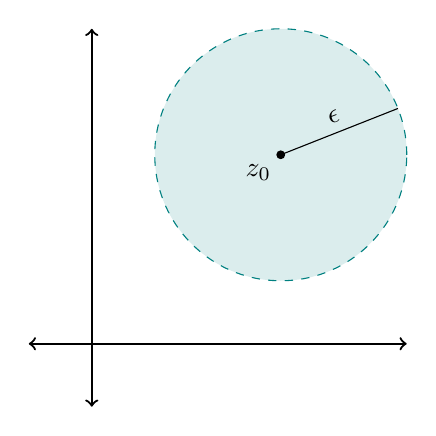
\begin{tikzpicture}[scale=0.8]
    \draw[<->,thick] (-1,0)--(5,0);
	\draw[<->,thick] (0,-1)--(0,5);
	\filldraw[teal,fill opacity=1/7,dashed](3,3) circle (2);
    \draw[](3,3)--(4.86,3.735) node[sloped,midway,above]{$\epsilon$};
    \fill (3,3) circle (2pt) node[below left]{$z_0$};
  \end{tikzpicture}
  \qquad\qquad\qquad
  \begin{tikzpicture}[scale=0.8]
    \draw[<->,thick] (-1,0)--(5,0);
	\draw[<->,thick] (0,-1)--(0,5);
	\filldraw[forest,fill opacity=1/7,dashed](3,3) circle (2);
    \draw[forest,dotted](3,3) circle (3pt);    
    \draw[](3,3)--(4.86,3.735) node[sloped,midway,above]{$\epsilon$};
    \fill[white] (3,3) circle (3pt) node[below left]{\color{black}$z_0$};
  \end{tikzpicture}\]
Points belonging to the same $\epsilon$-neighbourhood are considered "close" to each other, in the sense that they are within a distance of $2\epsilon$ from each other.
\end{definition}

\vspace*{1em}

\begin{definition}[Various kinds of Points]
Consider a $S \subseteq \cc$. 
\begin{itemize}
\item A point $z \in S$ is an \cdef{interior\ point\ of} {\color{blue}$S$} if there exists an $\epsilon > 0$ such that $D_\epsilon(z) \subseteq S$. 
\item A point $z \notin S$ is an \cdef{exterior\ point\ of} {\color{blue}$S$} if there exists an $\epsilon > 0$ such that $D_\epsilon(z) \cap S = \emptyset$. 
\item A point $z \in \cc$ is a \cdef{boundary\ point\ of} {\color{blue}$S$} if it's neither an interior nor an exterior point of $S$. Equivalently, if every neighbourhood of $z$ contains both a point in $S$ and not in $S$.
\item A point $z \in \cc$ is a \cdef{accumulation} (or \cdef{cluster}) \cdef{point\ of} {\color{blue}$S$} if for every $\epsilon > 0$ we have \[D_\epsilon(z)\setminus\set{z} \cap S \neq \emptyset.\]
\item A point $z \in S$ is an \cdef{isolated\ point\ of} {\color{blue}$S$} if there exists an $\epsilon > 0$ such that $D_\epsilon(z)\setminus\set{z} \cap S = \emptyset$. Isolated points are examples of boundary point
\end{itemize}
\[\begin{tikzpicture}[scale=1.1]
    \draw[<->,thick] (-2,0)--(5,0);
	\draw[<->,thick] (0,-2)--(0,5);
    \node[] at (4.75,2) {\color{dirt}$S$};
    
    \fill (3,4) circle (2pt) node[below]{\scriptsize$z_1$};
    \draw[](3,4)--(3.4,4.3) node[sloped,midway,xshift=-1pt,yshift=4pt]{\tiny$\epsilon_1$};
    \filldraw[indigo,fill opacity=1/10,dashed](3,4) circle (0.5);
    
    \fill (2.7,0.85) circle (2pt) node[below]{\scriptsize$z_2$};
    \draw[](2.7,0.85)--(3.45,0.85) node[sloped,midway,above,yshift=-1pt]{\tiny$\epsilon_2$};
    \filldraw[newblue,fill opacity=1/10,dashed](2.7,0.85) circle (0.75);
    
    \fill (-0.75,3.25) circle (2pt) node[below]{\scriptsize$z_3$};
    \draw[](-0.75,3.25)--(-1.75,3.25) node[sloped,midway,above,yshift=-1pt]{\tiny$\epsilon_3$};
    \filldraw[firebrick,fill opacity=1/10,dashed](-0.75,3.25) circle (1);
    
    \path[draw,use Hobby shortcut,closed=true,fill=dirt,fill opacity=1/10,dashed]
(-1,0) .. (3,0) .. (3,4) .. (1.5,2) .. (-1,0);
	\fill[dirt] (5,3) circle (2pt) node[below]{\scriptsize$z_4$};
\end{tikzpicture}\]
Here $z_1$ is a boundary point, $z_2$ an interior point, $z_3$ an exterior point, and $z_4$ is an isolated point (and a boundary point).
\end{definition}

%\vspace*{1em}

\begin{remark}
The idea is that if we don't move too far from an interior point of $S$ then we remain in $S$; a similar idea holds for an exterior point. But at a boundary point we can make an arbitrarily small move and get to a point inside $S$, and we can also make an arbitrarily small move and get to a point outside $S$. An accumulation point is one where it has other points from $S$ within any arbitrarily small distance, i.e. points "accumulate" near it; an isolated point is the exact opposite.
\end{remark}

\vspace*{2em}

\subsection{Problems}
\vspace*{0.1in}

\begin{problem}\label{prob 3.1}
Prove that 
\[\arg z + \arg w = \setp{(\parg z + \parg w) + 2k\pi}{k \in \zz}\]
Combining this with Proposition \ref{prodarg} we get that $\parg zw = \parg z + \parg w + 2k\pi$ for some $k \in \zz$ such that $-\pi < \parg z + \parg w + 2k\pi \leq \pi$. That is, to find $\parg zw$, just add $\parg z$ and $\parg w$ and then add or subtract a suitable multiple of $2\pi$ to get it between $-\pi$ and $\pi$.
\end{problem}

\vspace*{0.1in}

\begin{problem}\label{prob 3.2}
Prove that for any complex number $z$, we have $\parg \overline{z} = \parg z^{-1} = -\parg z$.
\end{problem}

\vspace*{0.1in}

\begin{problem}\label{prob 3.3}\hfill
\begin{itemize}
\item[(a)] Show that if $\Re z_1 > 0$ and $\Re z_2 > 0$, then $\parg(z_1z_2) = \parg z_1 + \parg z_2$.
\item[(b)] Show that if $\Re z > 0$, then $\parg(-z) = -\pi + \parg z$ if $\Im z > 0$ or $\parg(-z) = \pi + \parg z$ if $\Im z< 0$.
\item[(c)] Using (a) and (b), find an expression for $\parg zw$ for any non-zero complex numbers $z$ and $w$, in terms of $\parg z,\,\parg w$ and specific multiples of $\pi$.
\end{itemize}
\end{problem}

\vspace*{0.1in}

\begin{problem}\label{prob 3.4}
Compute the $6^{\text{th}}$ roots of unity, explicitly. Show that the principal $6^{\text{th}}$ root of unity is $\zeta_6 = -\omega$, where $\omega$ is as in Example \ref{cuberootofunity}.
\end{problem}

\vspace*{0.1in}

\begin{problem}\label{prob 3.5}\hfill
\begin{itemize}
\item[(a)] Let $z\in \cc$. Using the principle of mathematical induction, show that the following formula holds for all integers $n\geq 1$
\[1 + z + z^2 + \cdots + z^n = \frac{1-z^{n+1}}{1-z}.\]	
\item[(b)] Use (a) to derive \emph{Lagrange's Trigonometric Identity}.
\[1 + \cos\theta + \cos^2\theta + \cdots + \cos^n\theta = \frac{2\sin((2n+1)\theta/2)}{2\sin(\theta/2)},\quad 0 < \theta < 2\pi.\]
\item[(c)] If $\zeta_1,\ldots,\zeta_n$ are the \emph{distinct} $n^{\text{th}}$ roots of unity, show that, using (a), $\displaystyle \sum_{i=1}^n \zeta_i = 0$.
\item[(d)] We compute the following sum of real numbers
\begin{equation*}\label{trigsum}
\cos \frac{\pi}{7} + \cos \frac{3\pi}{7} + \cos \frac{5\pi}{7} \tag{$\dagger$}
\end{equation*}
\begin{itemize}[itemsep=1em]
\item[(i)] Let $w = e^{\frac{\pi i}{7}}$. What is $\Re w$ and $w^7$? Furthermore, rewrite (\ref{trigsum}) as
\[\Re(w^{a_1} + w^{a_2} + w^{a_3}),\quad \text{for some $0 \leq a_i < 7$.}\]
\item[(ii)] Replacing $z$ by $-z$ in (a), find a formula for \[\dfrac{z^7 + 1}{z + 1}.\]
Use this to deduce an identity involving $w$ and its powers.
\item[(iii)] Using the identity you found in (iii), conclude that 
\[w^{a_1} + w^{a_2} + w^{a_3} = \frac{1}{1-w}\]
where the $a_i$'s are the numbers you found in (ii).
\item[(iv)] Finally compute (\ref{trigsum}).
\end{itemize}
\end{itemize}
\end{problem}